\chapter{Avancement par tâche}

Les différentes avancées depuis la dernière revue de projet sont expliquées ici sans rentrer dans les détails techniques. Ceux-ci figureront dans le rapport de l'évaluation finale.

\section{Hardware}

Le circuit imprimé a été fabriqué sans encombre. Il est actuellement en cours de validation.

\begin{itemize}[label=$\bullet$]
	\item Aucune fuite de courant ni discontinuité de piste.
	\item Le convertisseur $12V/5V$ est opérationnel.
	\item La protection aux surtensions l'est également.
	\item L'environnement des interrupteurs de butée n'a pas encore été testé.
	\end{itemize}

\begin{figure}[H]
    \centering
	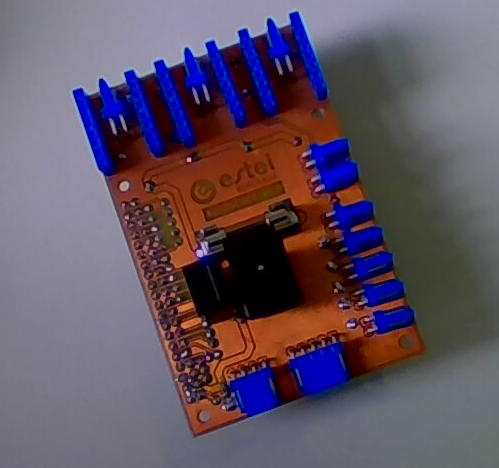
\includegraphics[width=0.32\linewidth]{\figures/photo_hardware1.png}
	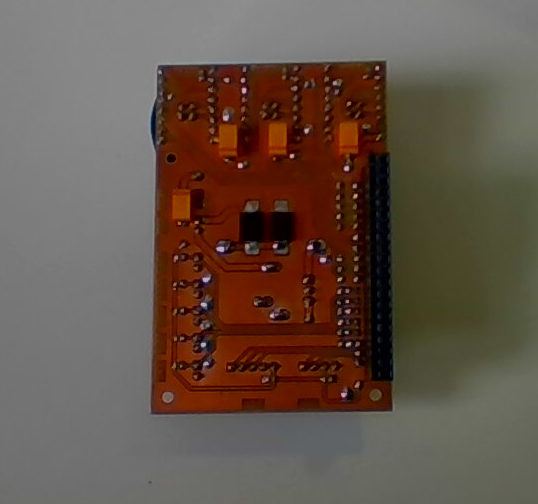
\includegraphics[width=0.32\linewidth]{\figures/photo_hardware3.png}
	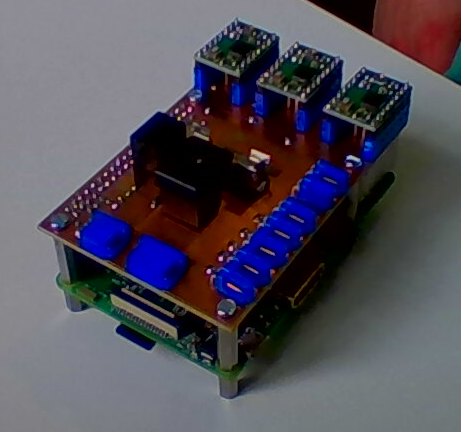
\includegraphics[width=0.32\linewidth]{\figures/photo_hardware2.png}
    \decoRule
    \caption[
    Photos du circuit imprimé du télescope]{
    Photos du circuit imprimé du télescope}
    \label{fig:Photos du circuit imprimé du télescope}
    \end{figure}

\section{Système d'exploitation}

La configuration du hotspot Wifi a été rétablie, il s'agissait d'une erreur discrète dans un fichier de configuration de \codeinline{text}{connman}. Voici donc un aperçu de la connexion au télescope depuis un ordinateur distant, ainsi que du serveur FTP qui redevient par là même utilisable.

\begin{figure}[H]
    \centering
    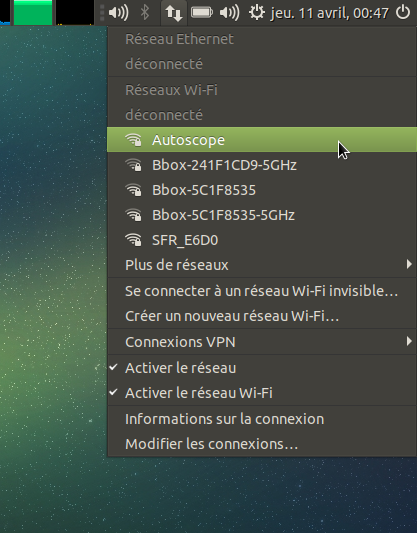
\includegraphics[width=0.4\linewidth]{\figures/photo_hotspot.png}
    \decoRule
    \caption[
    Connexion à la Raspberry-Pi depuis un ordinateur distant]{
    Connexion à la Raspberry-Pi depuis un ordinateur distant}
    \label{fig:Connexion à la Raspberry-Pi depuis un ordinateur distant}
    \end{figure}

\begin{figure}[H]
    \centering
    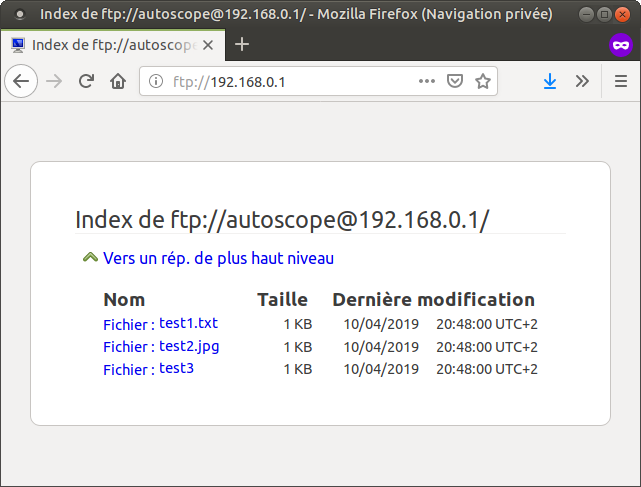
\includegraphics[width=0.7\linewidth]{\figures/photo_ftp.png}
    \decoRule
    \caption[
    Accès au serveur FTP de la Raspberry-Pi depuis un navigateur]{
    Accès au serveur FTP de la Raspberry-Pi depuis un navigateur}
    \label{fig:Accès au serveur FTP de la Raspberry-Pi depuis un navigateur}
    \end{figure}

\vspace{1cm}

De plus le support de la liaison UART et du bus I2C ont été activé. Ci dessous des trames relevées à l'analyseur logique pour chaque protocole. La trame I2C n'est pas acquittée car aucun périphérique n'est présent pour le faire, il s'agit d'une trame d'adresse envoyée dans le vide par la Raspberry-Pi.

\begin{figure}[H]
    \centering
    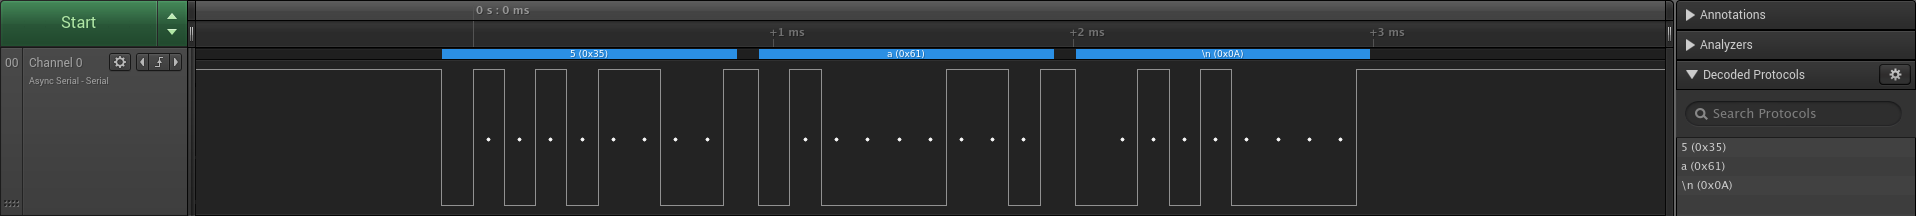
\includegraphics[width=1\linewidth]{\figures/osc_uart.png}
    \decoRule
    \caption[
    Trame UART relevée à l'analyseur logique]{
    Trame UART relevée à l'analyseur logique}
    \label{fig:Trame UART relevée à l'analyseur logique}
    \end{figure}

\begin{figure}[H]
    \centering
    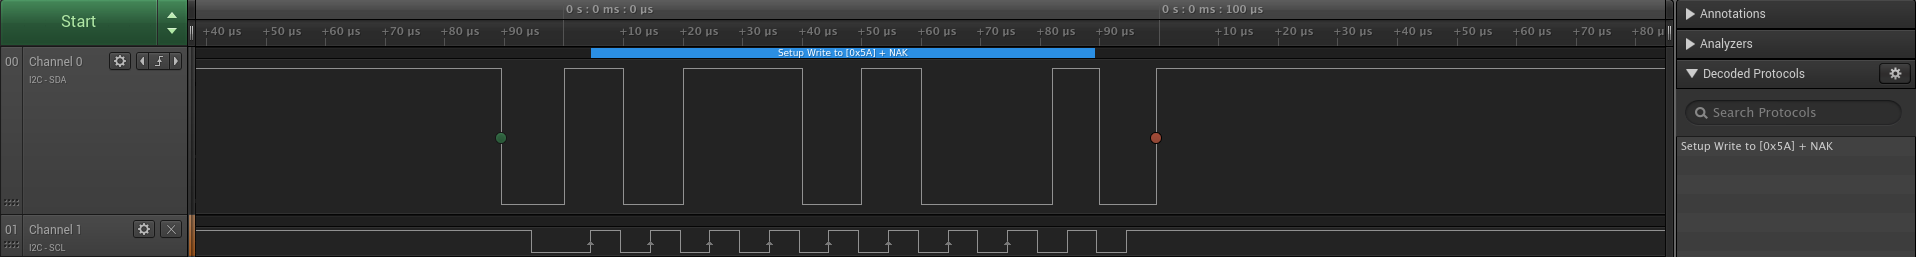
\includegraphics[width=1\linewidth]{\figures/osc_i2c.png}
    \decoRule
    \caption[
    Trame I2C relevée à l'analyseur logique]{
    Trame I2C relevée à l'analyseur logique}
    \label{fig:Trame I2C relevée à l'analyseur logique}
    \end{figure}

\section{Communication inter-processus}

Cette partie consiste à rendre le driver accessible à l'application principal du système. Pour cela j'utilise la manière qui utilise \codeinline{text}{ioctl()}. Le moyen technique utilise des fichiers virtuels en lecture/écriture entre l'espace utilisateur (user-space, dans lequel il y aura l'application) et la couche kernel (dans laquelle il y a les drivers d'accessible). Via ce fichier les ordres sont envoyés au driver.
Un code utilisant l'\codeinline{text}{ioctl} à été validé, l'implémentation dans le driver de contrôle des moteurs est bientôt finie.

\begin{figure}[H]
    \centering
	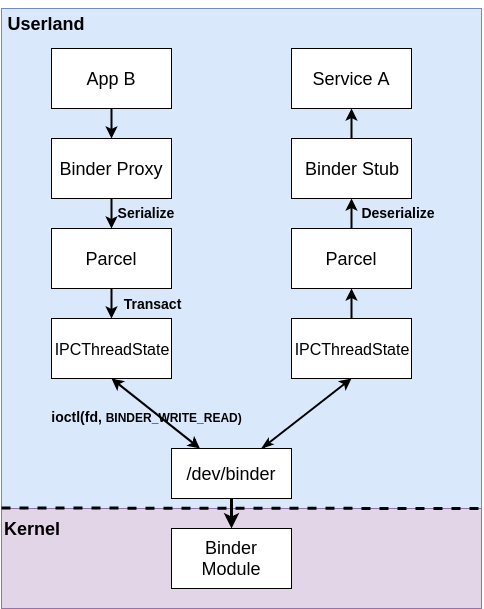
\includegraphics[width=0.49\linewidth]{\figures/binder_layers.png}
    \decoRule
    \caption[
    Schéma des couches lors de la communication app/driver]{
    Schéma des couches lors de la communication app/driver}
    \label{fig:Schéma des couches lors de la communication app/driver}
    \end{figure}

\section{Stellarium}

La procédure de compilation de Stellarium ainsi que de ses dépendances a été étudiée et détaillée dans le \codeinline{text}{README} du dépôt du plugin produit par Thibaud LE DOLEDEC.

\url{https://github.com/thibaudledo/Autoscope-Stellarium-plugin}

\vspace{1cm}

Le plugin devient alors accessible et utilisable. La procédure permet en particulier de livrer des paquets binaires pré-compilés d'une version de Stellarium intégrant le plugin, qu'il ne reste alors qu'à installer comme n'importe quel logiciel. Un paquet compilé pour Linux est disponible ici~: \url{https://github.com/thibaudledo/Autoscope/releases}

\vspace{1cm}

Ci-dessous un aperçu de l'interface de l'interface qu'offre le plugin~:

\begin{figure}[H]
    \centering
	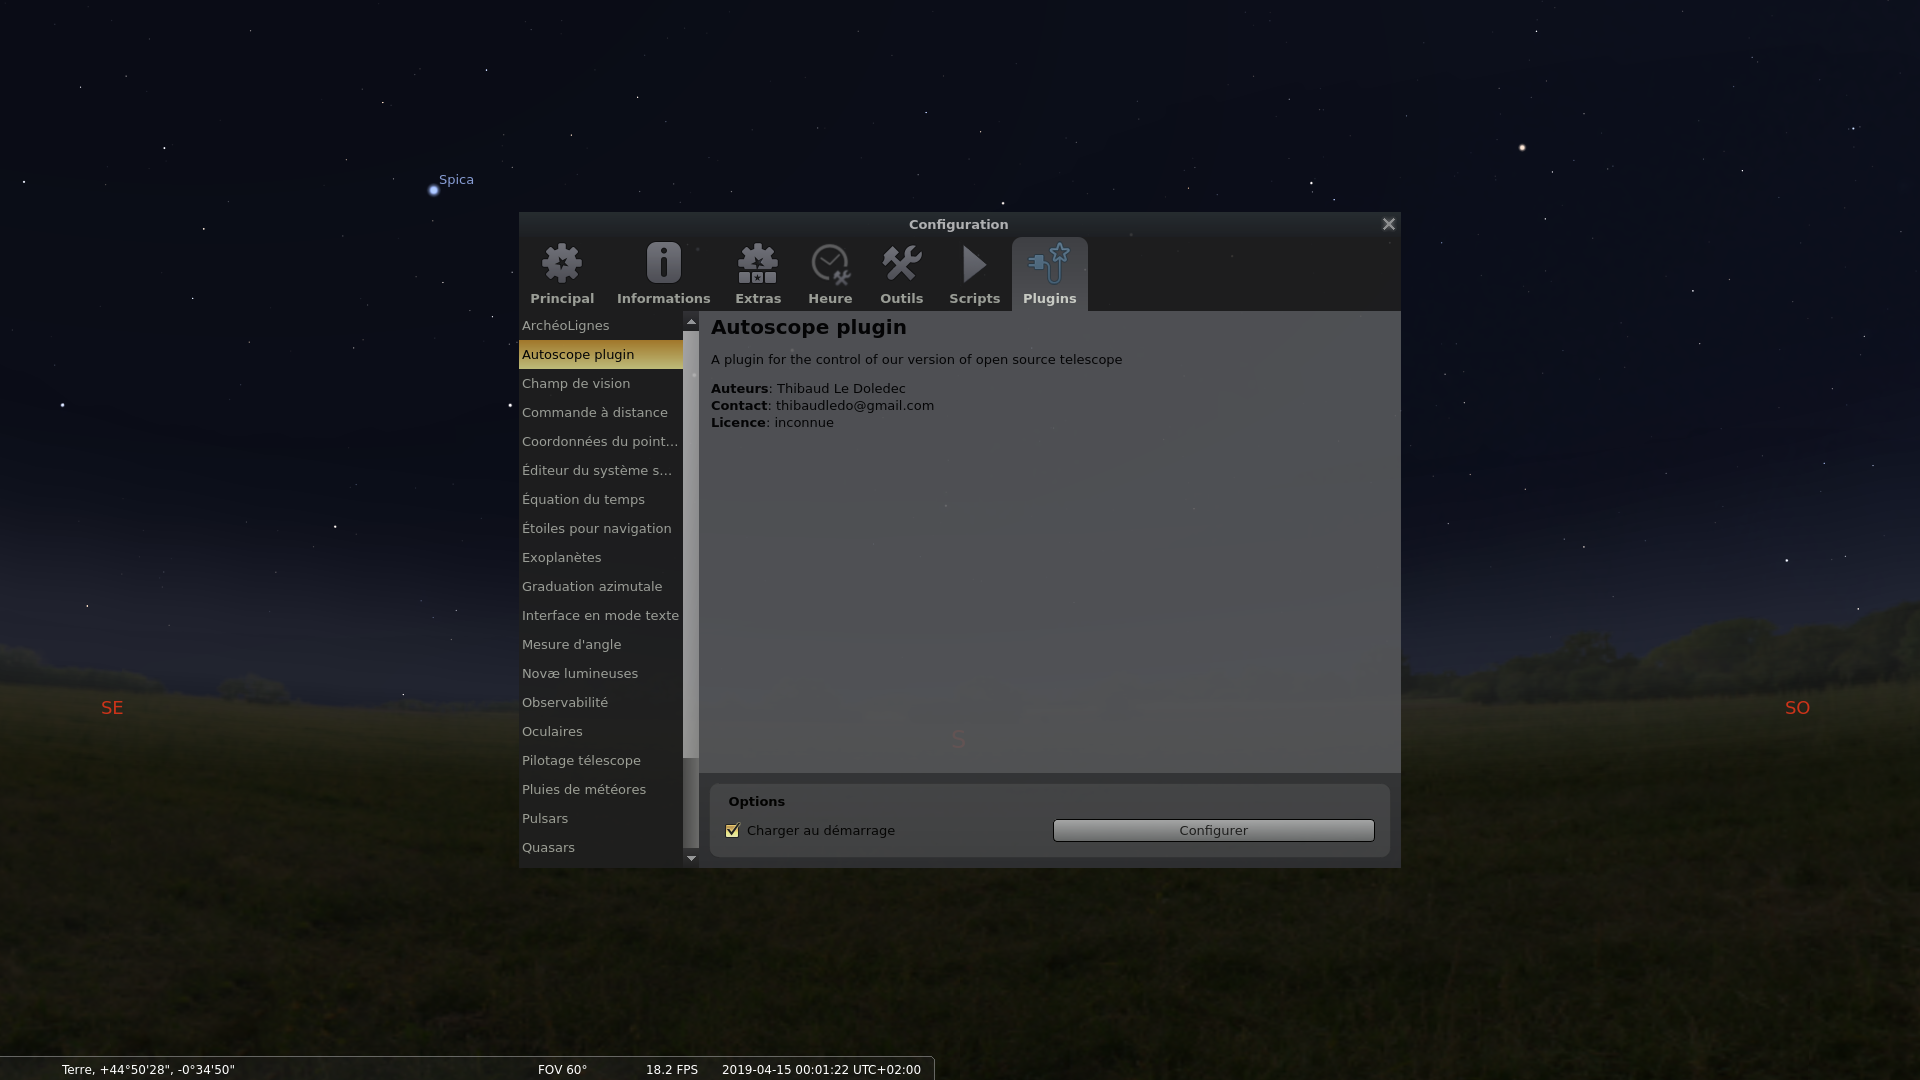
\includegraphics[width=0.9\linewidth]{\figures/photo_stellarium1.png}
	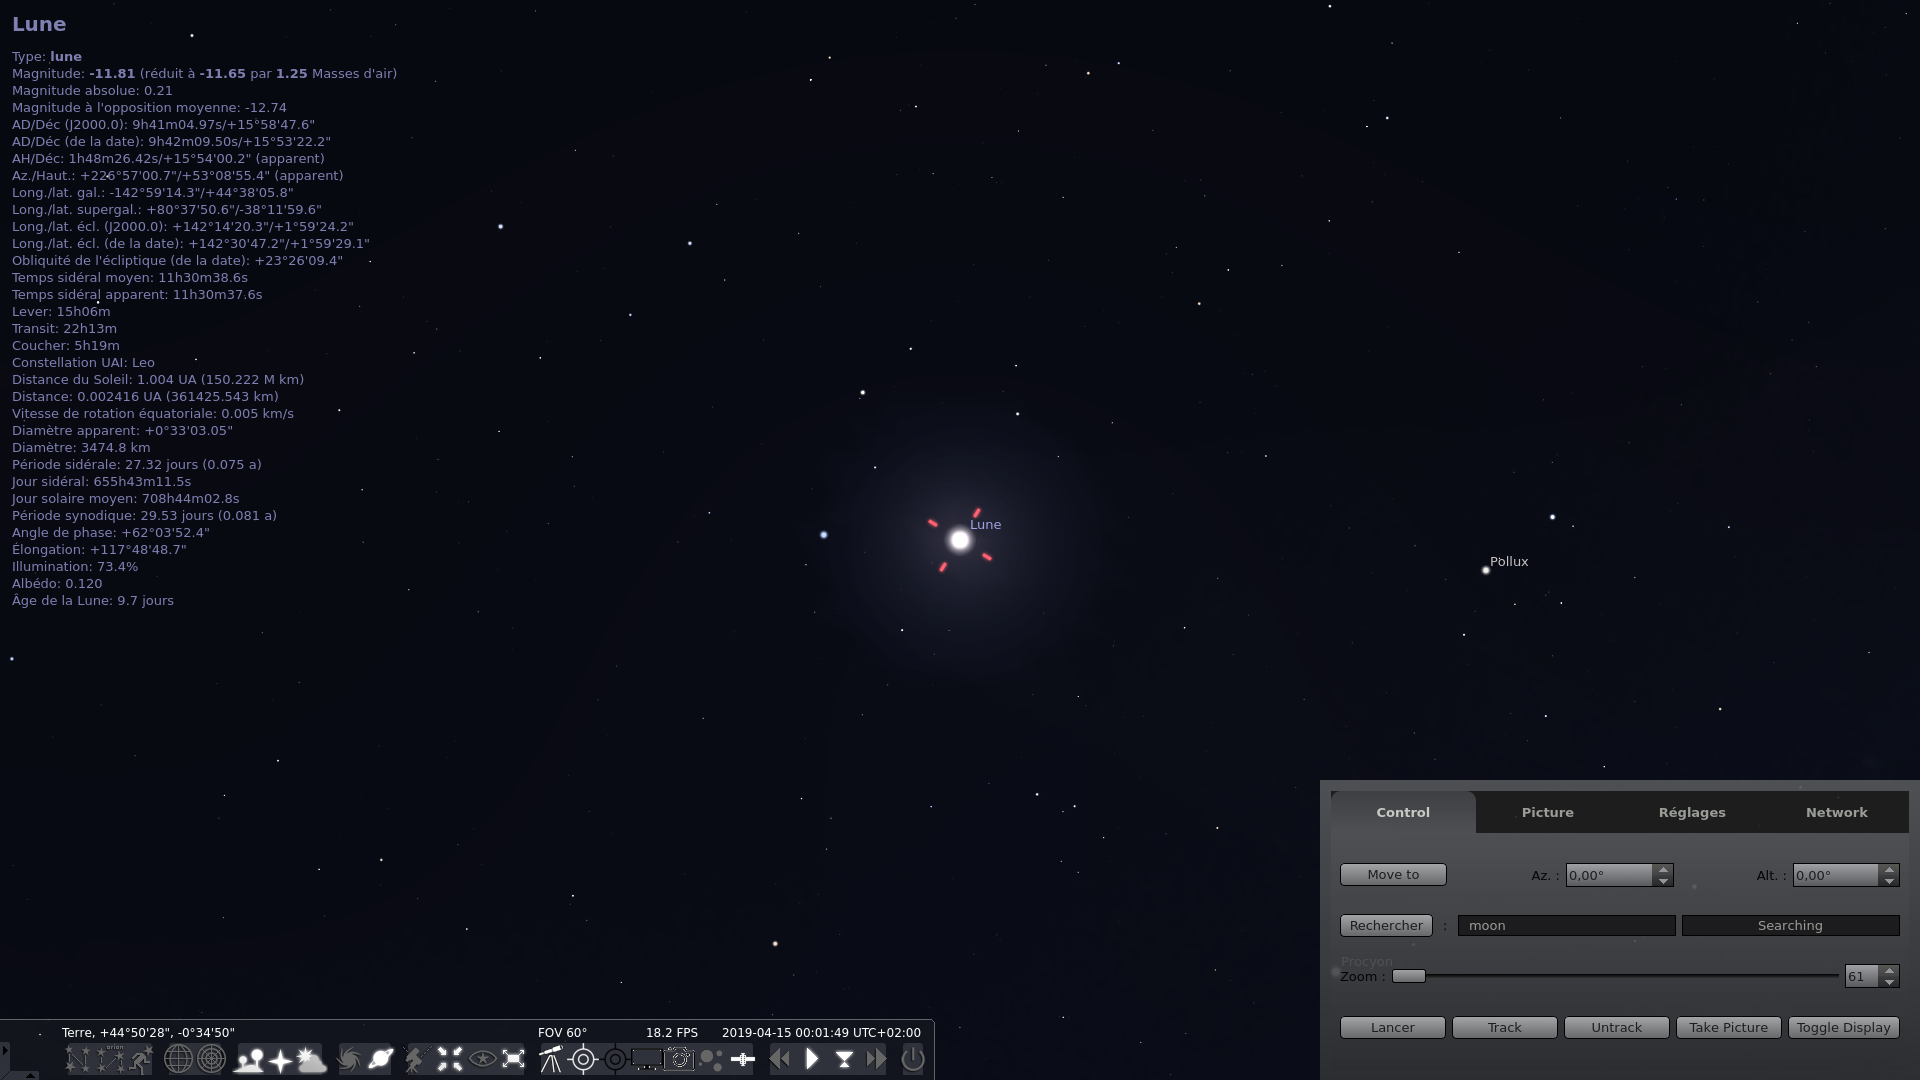
\includegraphics[width=0.9\linewidth]{\figures/photo_stellarium2.png}
    \decoRule
    \caption[
    Aperçu de l'interface du plugin Stellarium]{
    Aperçu de l'interface du plugin Stellarium}
    \label{fig:Aperçu de l'interface du plugin Stellarium}
    \end{figure}
